\documentclass[utf-8]{ctexart}
\usepackage{a4}
\usepackage{listings}
\usepackage{amsmath,amssymb}
\usepackage{parskip}
\usepackage{graphicx}
\usepackage{indentfirst}%设置锁进
\usepackage[top=2.5cm, left=3cm, right=3cm, bottom=4.0cm]{geometry}

\title{设计文稿}
\author{计92 高敬越 2019011230}

\setlength{\parindent}{2em}

\begin{document}
    \maketitle
    \section{环境}
    \begin{enumerate}
        \item 系统: macOS 10.15.6
        \item Qt版本:Qt 5.15.0 clang 64bit 
    \end{enumerate}
    \section{功能介绍}

    \subsection{游戏界面与各个状态}

    \begin{figure}[ht]
        \centering
        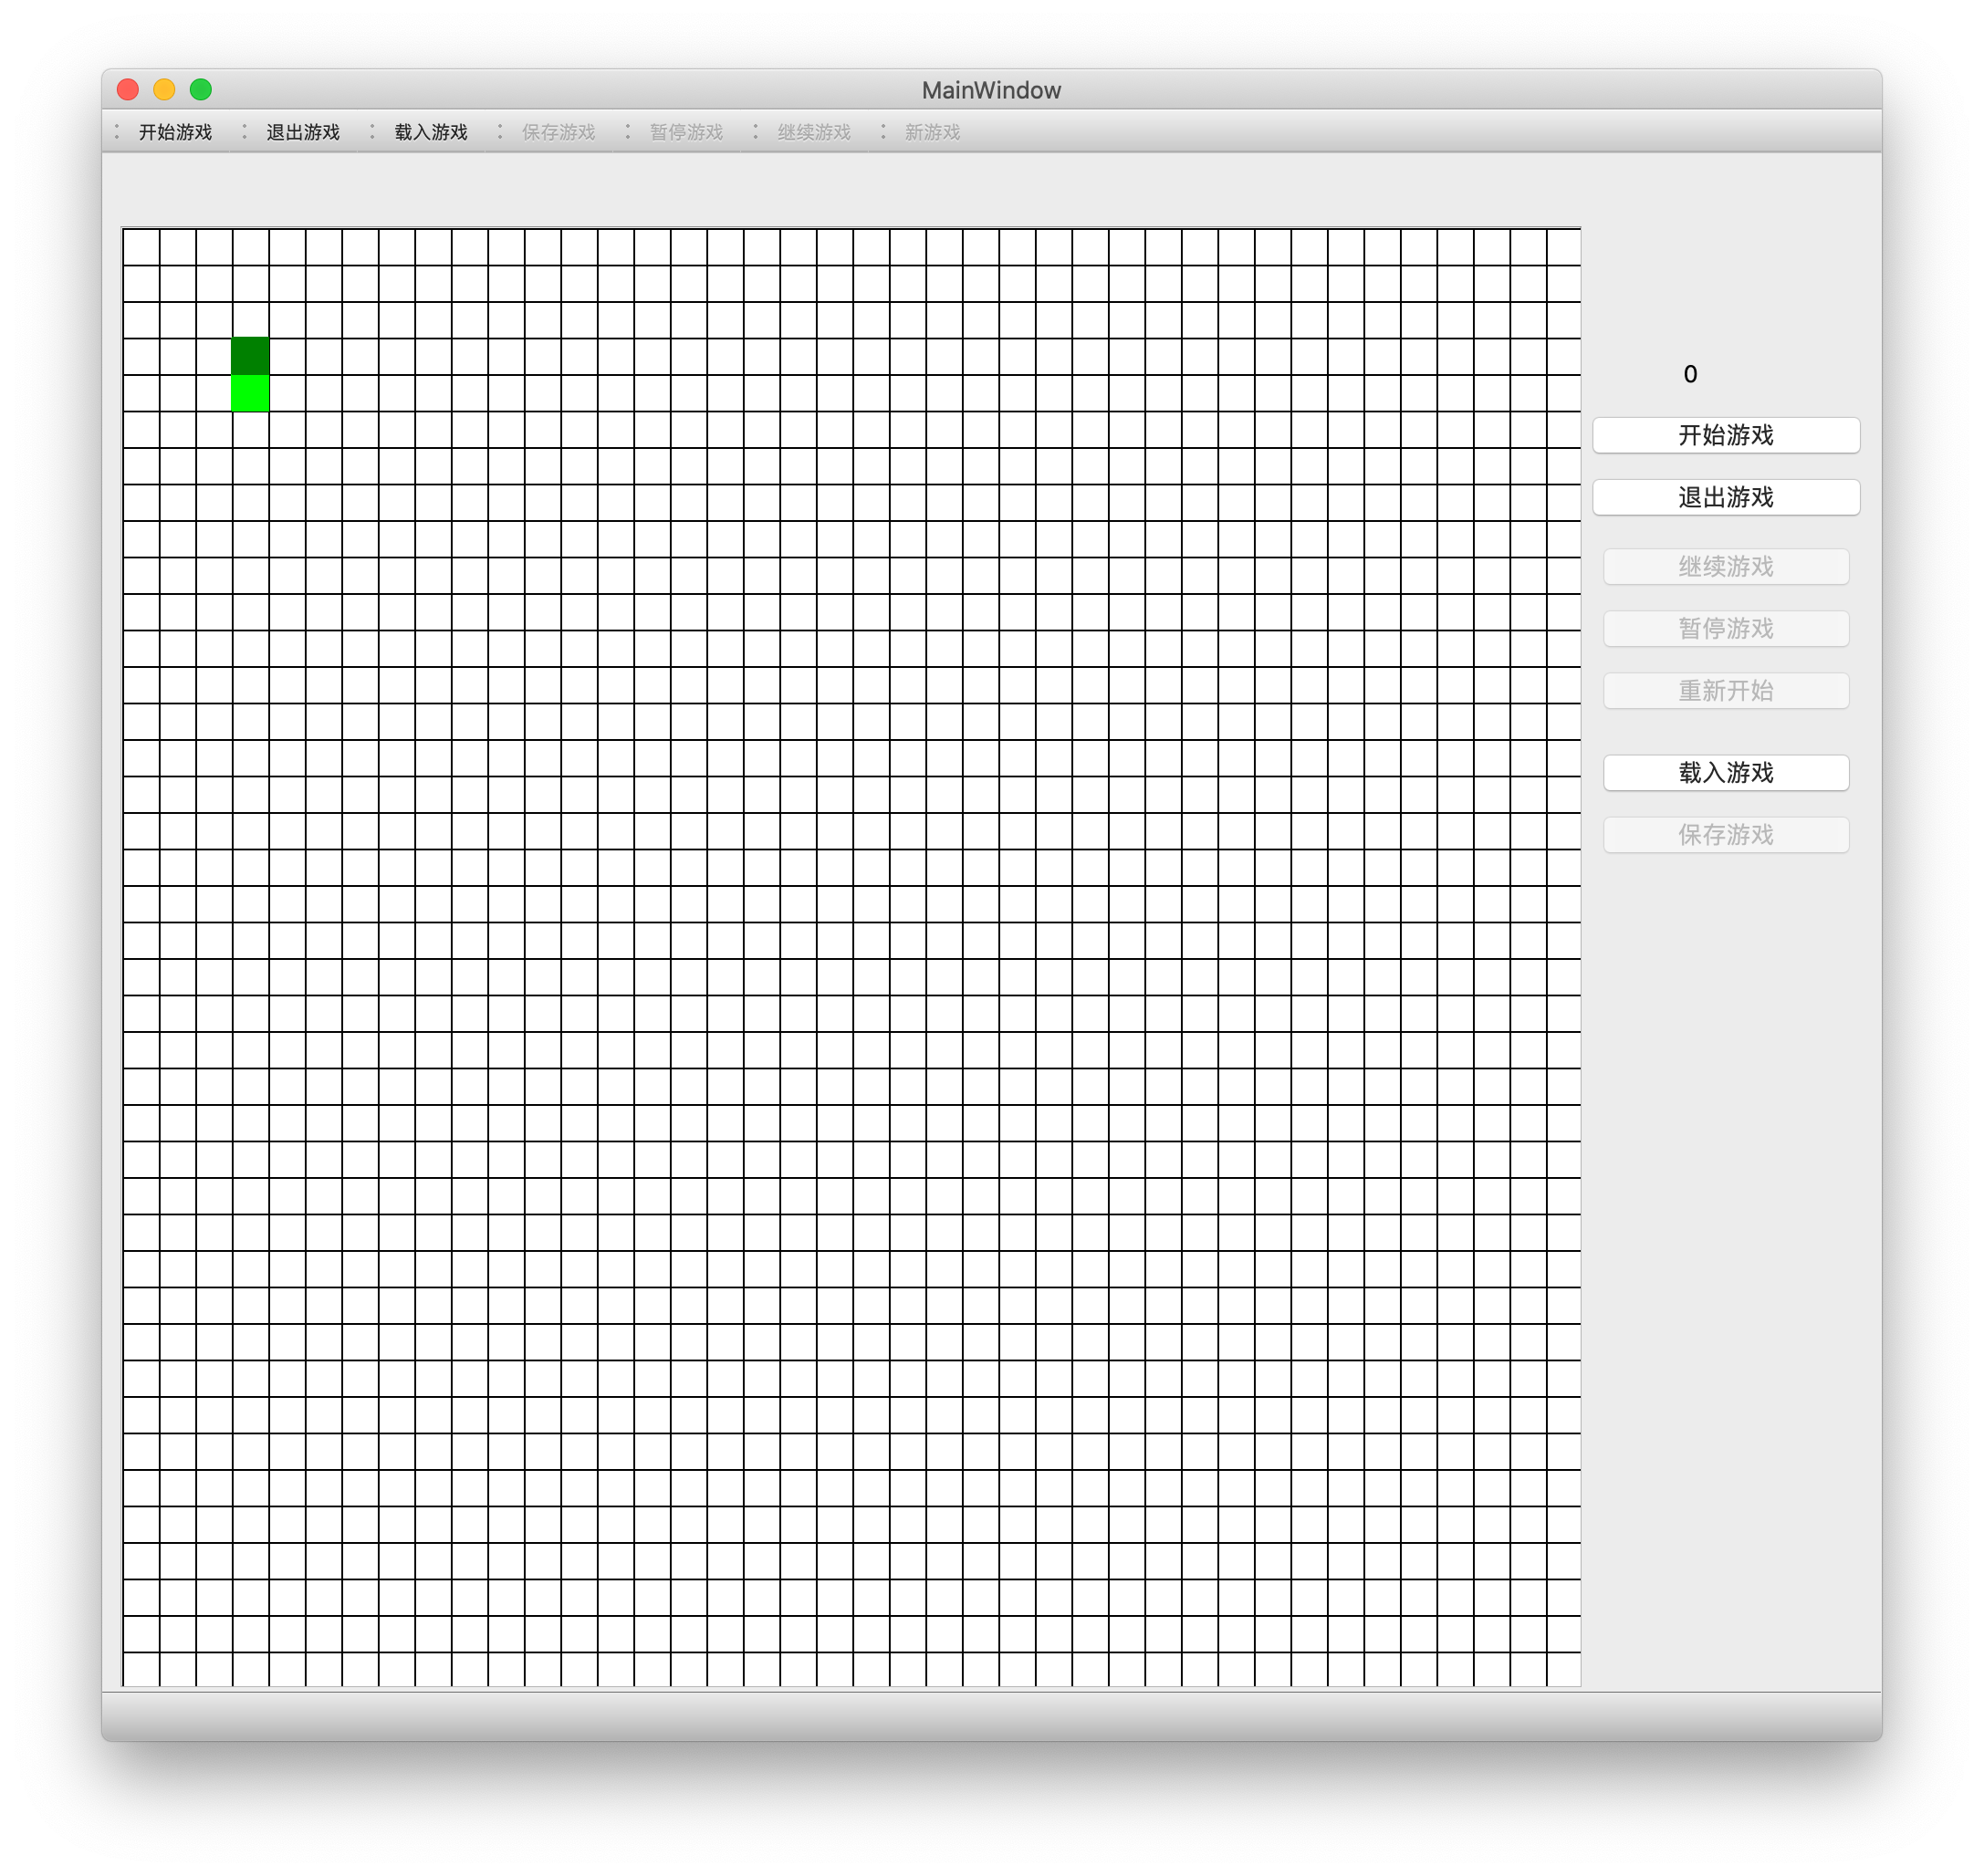
\includegraphics[scale = 0.2]{texsrc/界面.png}
        
\includegraphics[scale = 0.4]{texsrc/菜单栏.png}
        \caption{未开始状态的界面}
        \label{intialized}
    \end{figure}
    \begin{figure}[ht]
        \centering
        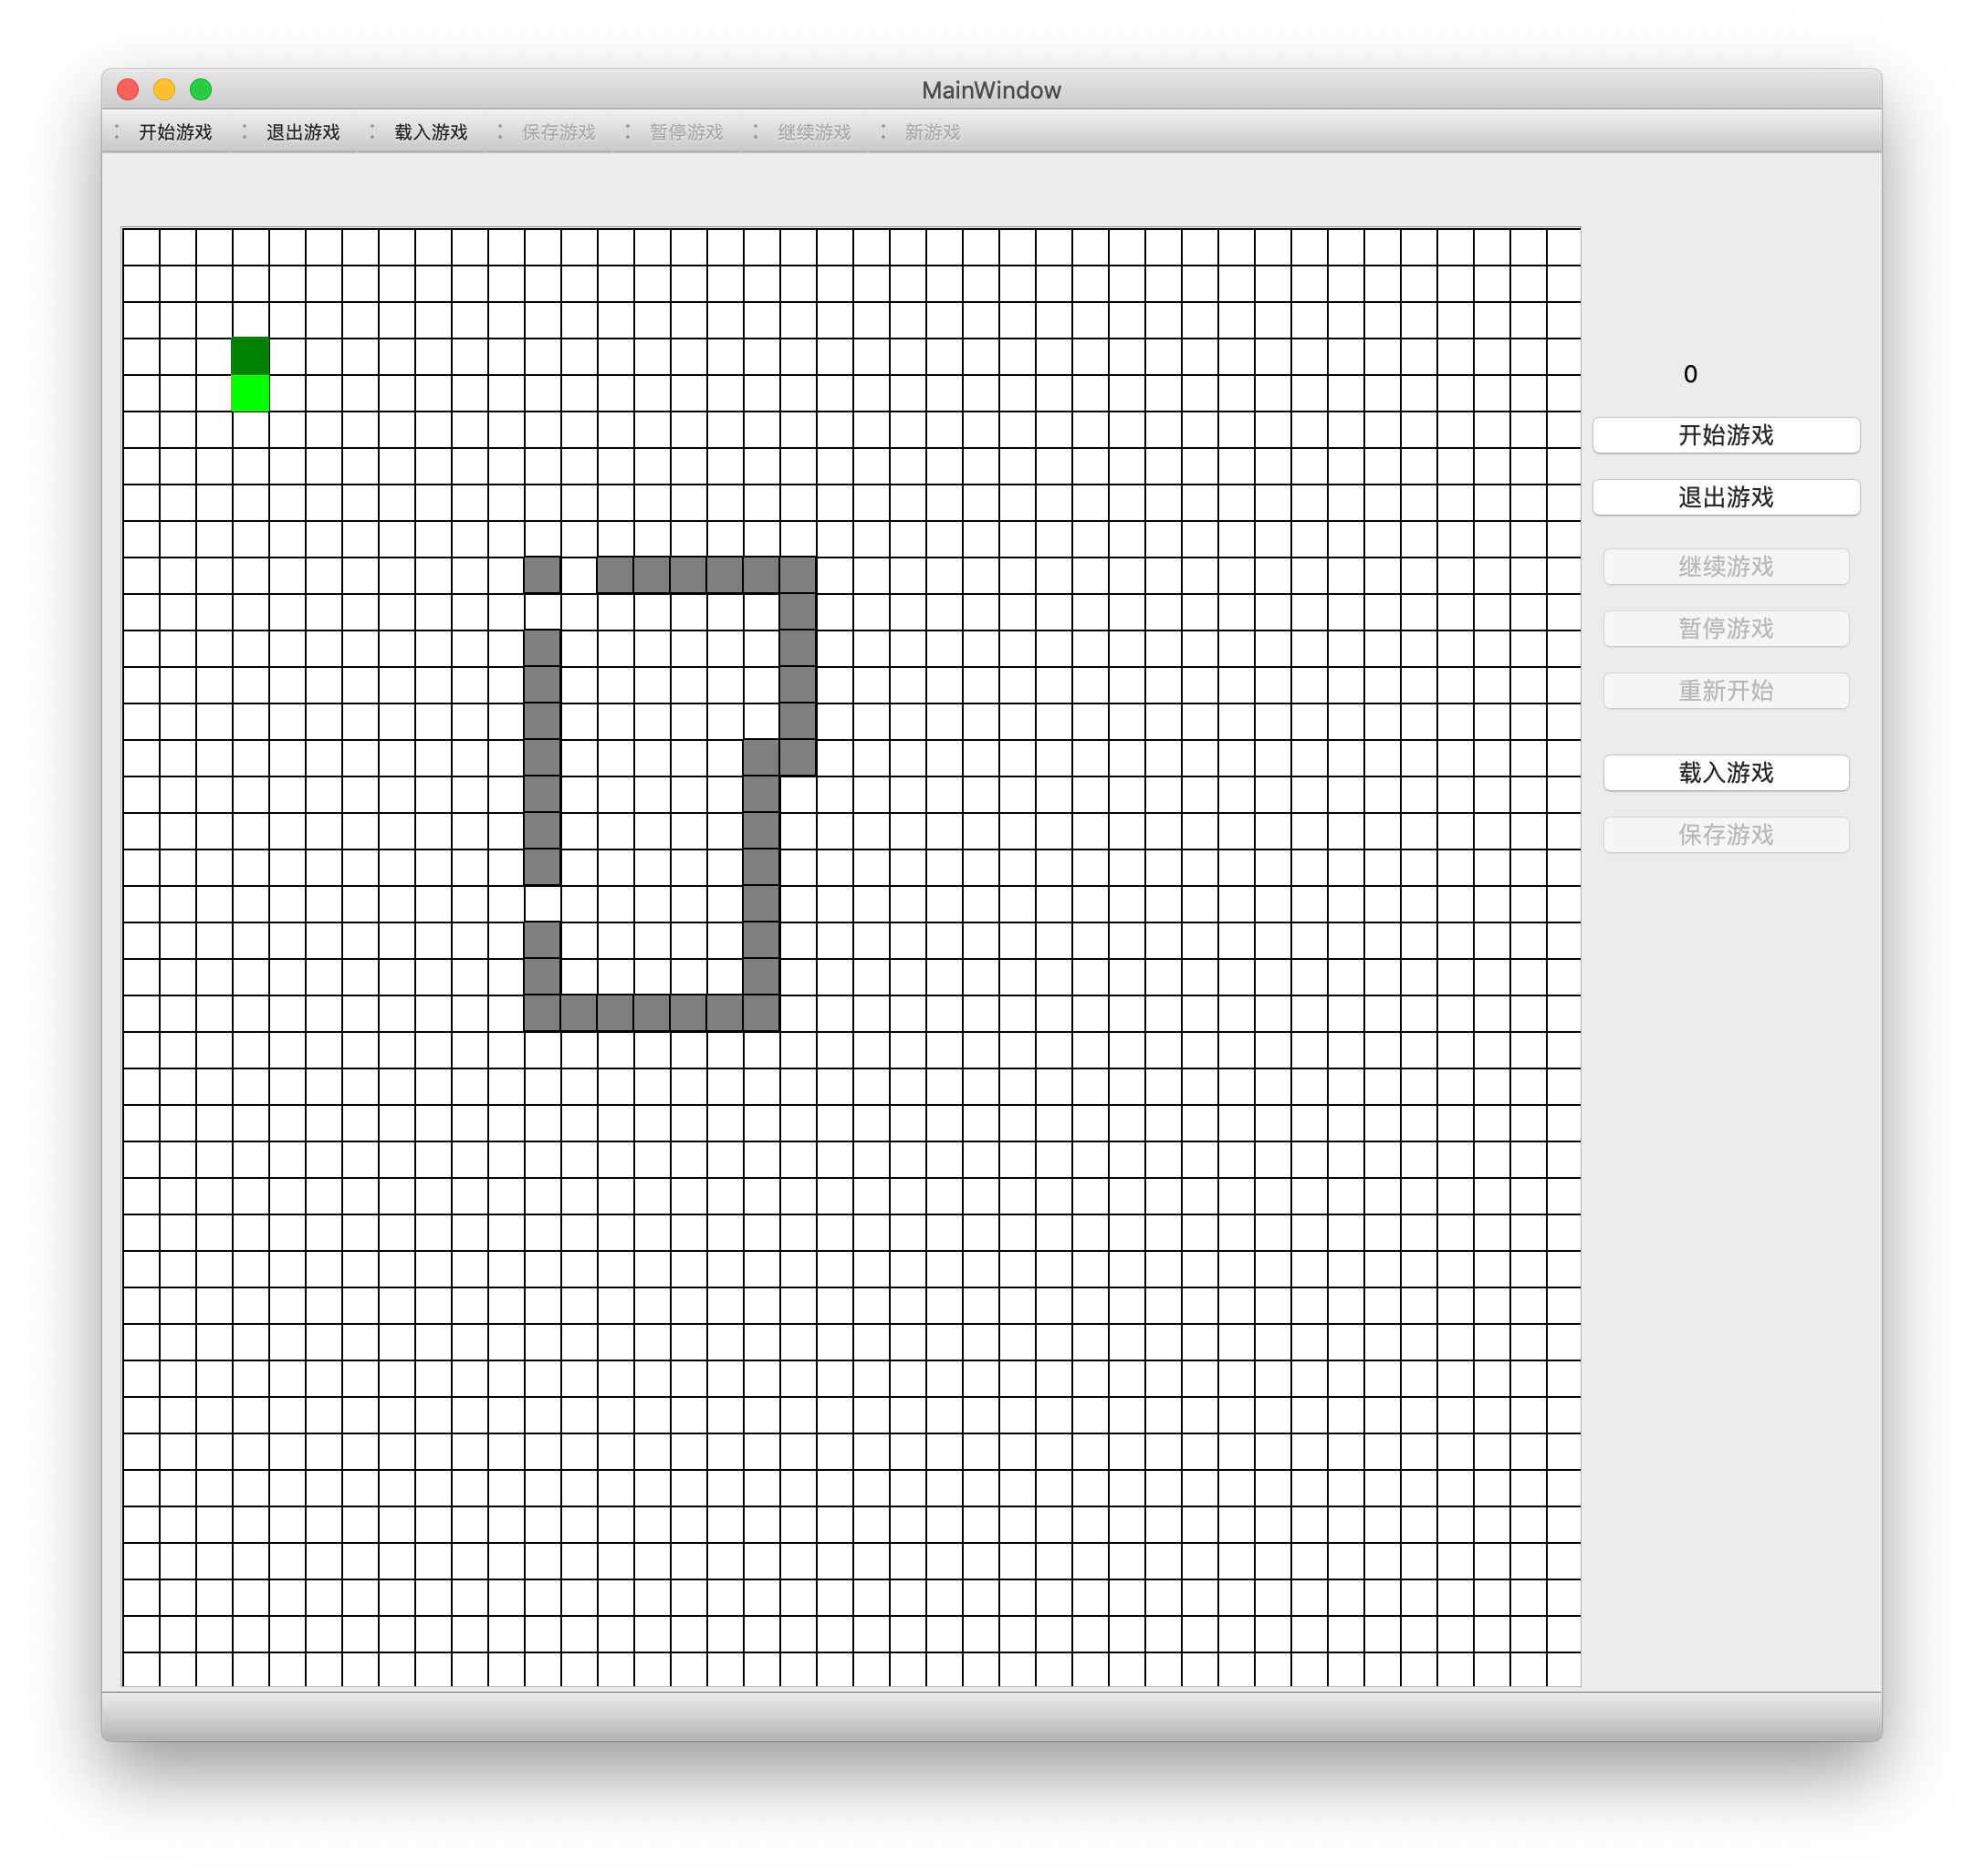
\includegraphics[scale = 0.2]{texsrc/界面+wall.png}
        \caption{点击网格,增加障碍}
        \label{obstacle}
    \end{figure}
    \par 图1为已初始化、未开始状态时的游戏界面。(由于macOS的特点,应用的菜单栏单独在屏幕最上面)图1上的图是包含工具栏、按钮、时间展示以及游戏区的主界面,
    图1下为菜单栏。\par 在菜单栏中,“操作”菜单中包含开始游戏、结束游戏两个功能,“保存/载入”菜单中包含保存游戏、载入游戏两个功能,“游戏操作”
    菜单中包含暂停游戏、继续游戏、重新开始三个操作。(具体点开的截图略)\par 在主界面中,最上方一行为工具栏,同样实现了上述的
    所有操作;右侧最上方数字显示时间,大小与蛇走过的距离相同;右侧下方的按钮分别对应了以上所有操作,同时也
    满足了在未开始状态只有开始游戏、退出游戏、载入游戏处于可用状态。主界面中间是40*40格的游戏界面,并初始化了长度为2的蛇(蛇头为深绿色,身体为浅绿色),
    默认运动方向向上。同时在此阶段,可以点击方格来设置障碍,障碍以与各自同样大小的灰色正方形表示(如图2);在增加后,也支持再次点击以消除障碍。

    \begin{figure}[ht]
        \centering
        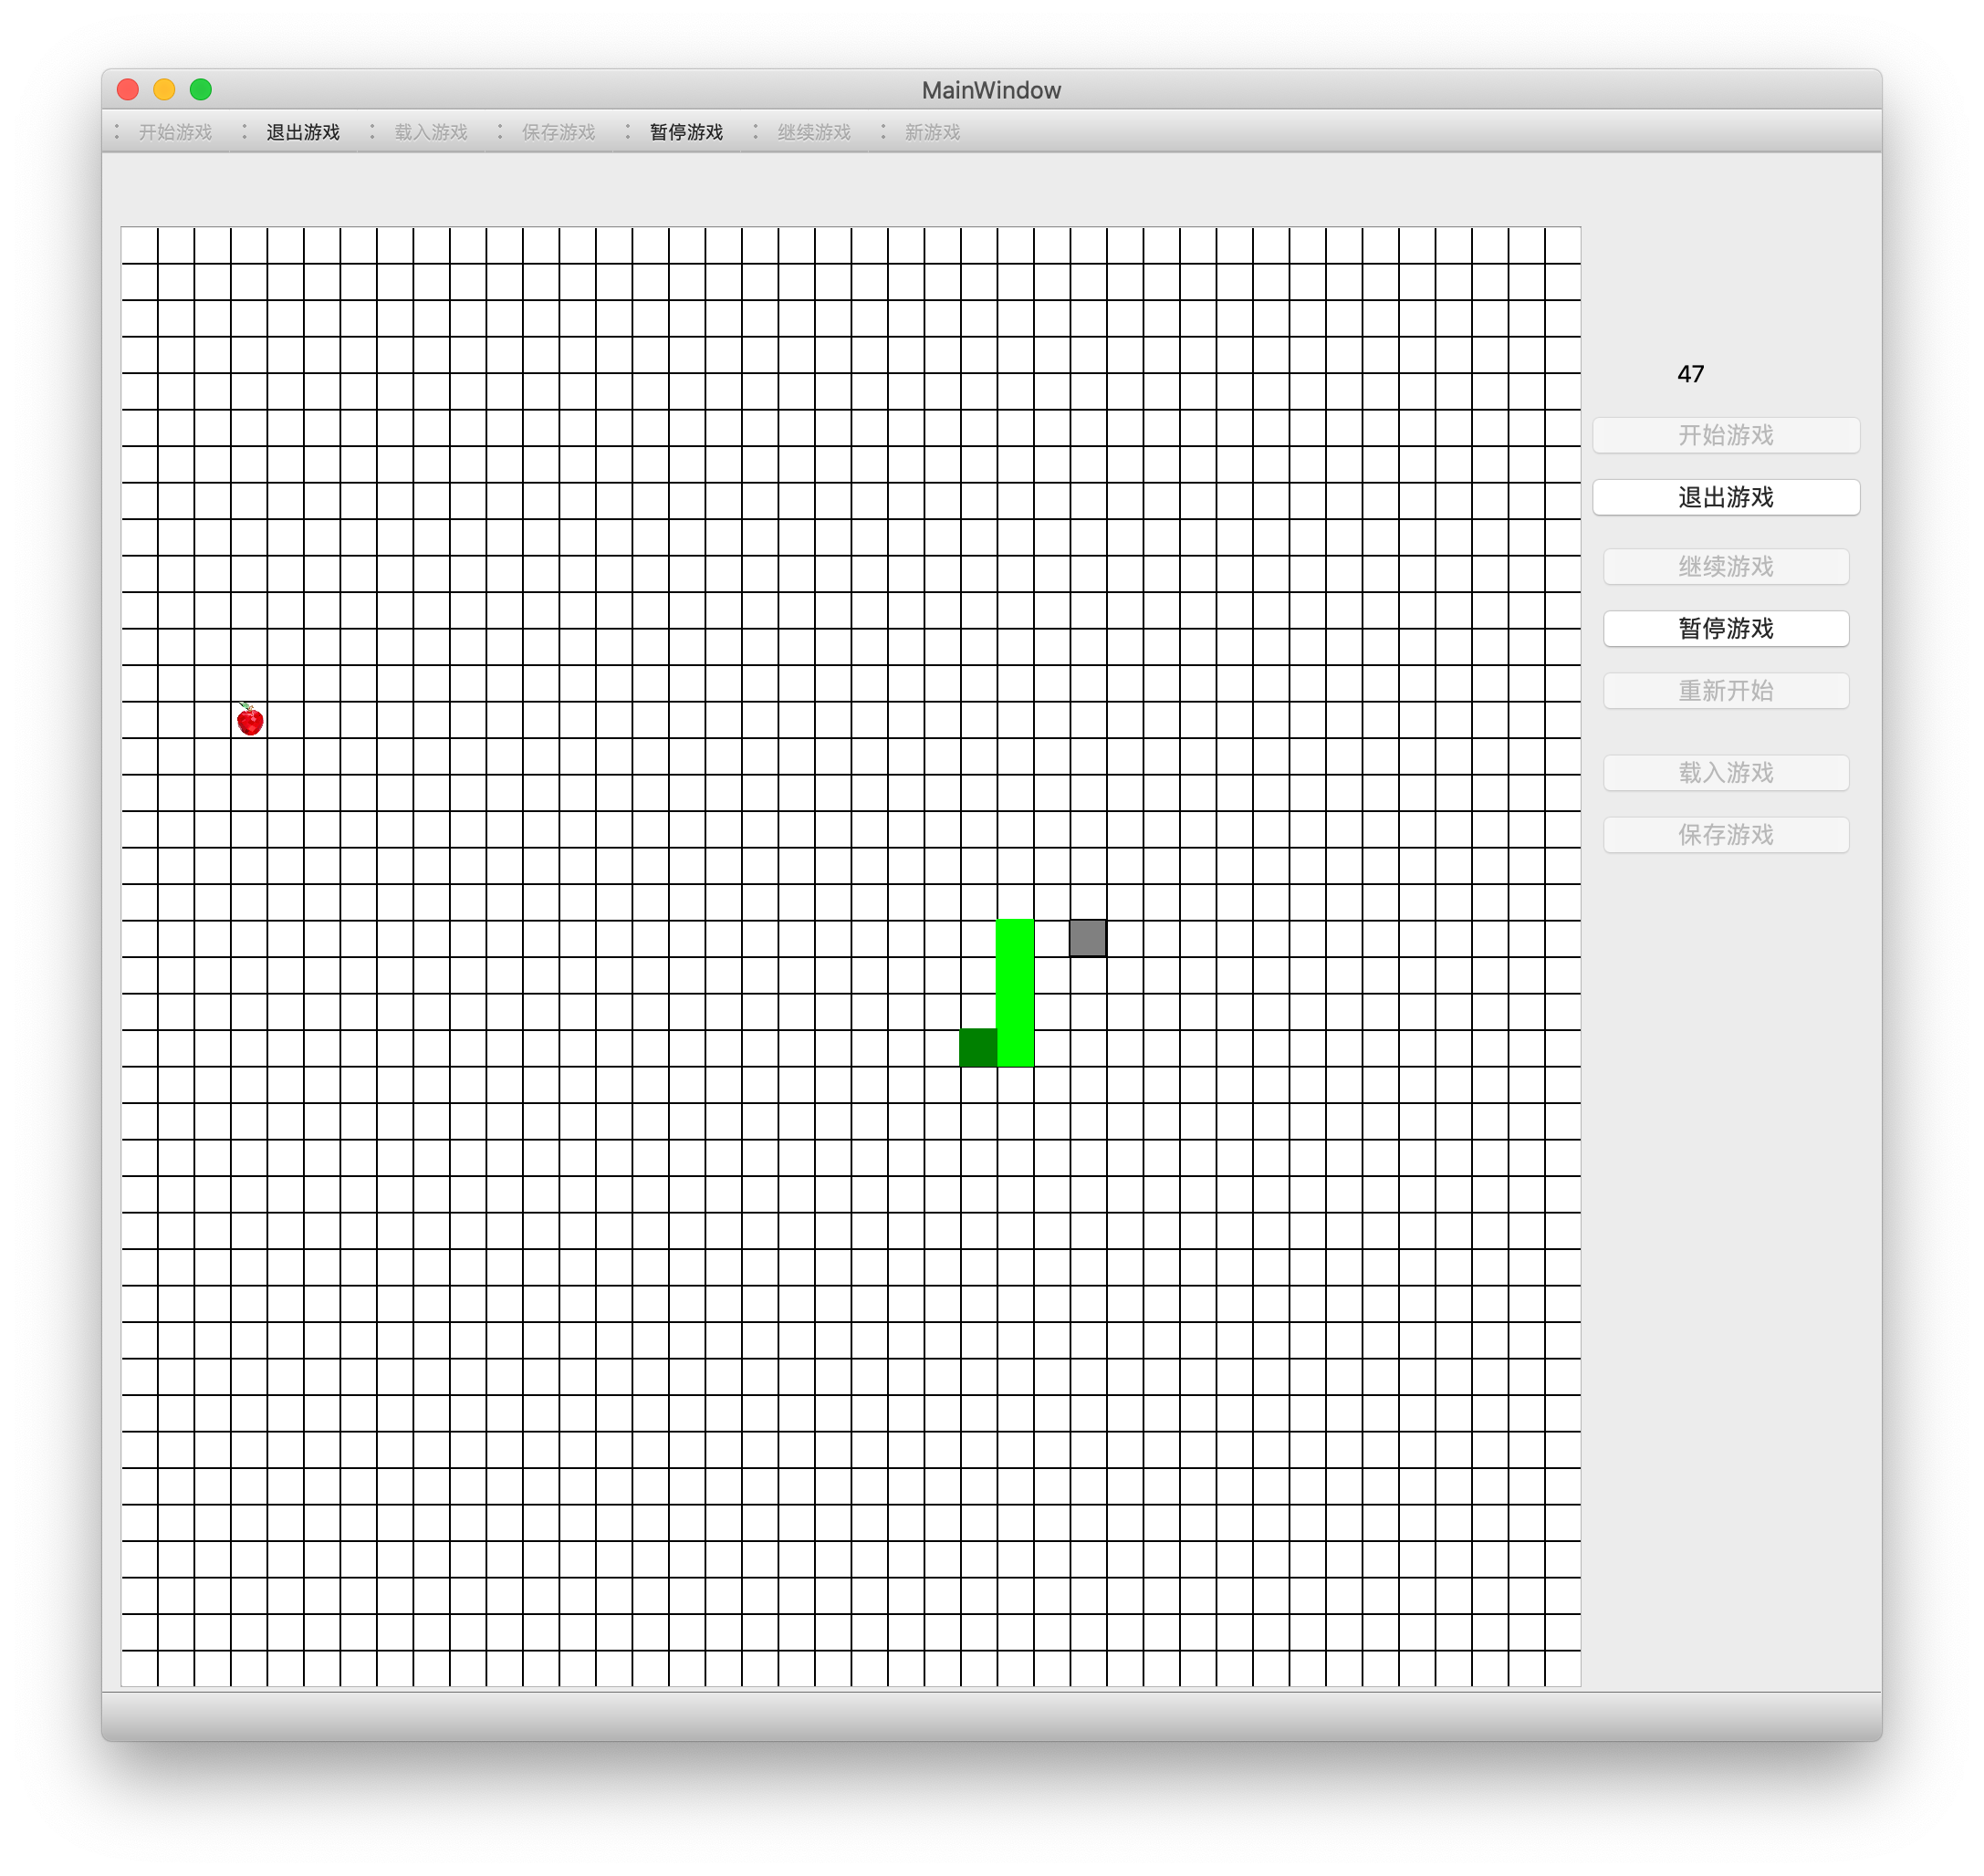
\includegraphics[scale = 0.3]{texsrc/开始游戏.png}
        \caption{游戏状态}
        \label{gaming}
    \end{figure}
    \par 点击开始游戏后,贪吃蛇开始移动,同时随机产生一个食物(图标为小苹果)。
\end{document}